\documentclass[a4paper,11pt]{article}
\usepackage[cm]{fullpage}
\usepackage{bchart}
\usepackage{pgfplots}
\usepackage{listings}
\usepackage[colorinlistoftodos]{todonotes}

\title{MLAP Open Assessment}
\author{Y6186228}
\date{14th May 2014}

\pgfplotsset{compat=1.10}

\newcommand*{\foa}[1]{f(\theta) = \theta_0 + \theta_1 {#1}}
\newcommand*{\fa}[1]{$\foa{#1}$}

\newcommand*{\fob}[2]{f(\theta) = \theta_0 + \theta_1 {#1} + \theta_2 {#2}}
\newcommand*{\fb}[2]{$\fob{#1}{#2}$}

\newcommand*{\foc}[3]{f(\theta) = \theta_0 + \theta_1 {#1} + \theta_2 {#2} + \theta_3 {#3}}
\newcommand*{\fc}[3]{$\foc{#1}{#2}{#3}$}

\newcommand*{\fod}[4]{f(\theta) = \theta_0 + \theta_1 {#1} + \theta_2 {#2} + \theta_3 {#3} + \theta_4 {#4}}
\newcommand*{\fd}[4]{$\fod{#1}{#2}{#3}{#4}$}

\newcommand*{\foe}[5]{f(\theta) = \theta_0 + \theta_1 {#1} + \theta_2 {#2} + \theta_3 {#3} + \theta_4 {#4} + \theta_5 {#5}}
\newcommand*{\fe}[5]{$\foe{#1}{#2}{#3}{#4}{#5}$}

\begin{document}
\maketitle

\section{Linear regression and Logistic regression}
\label{s1}
\subsection{Task 1}
\label{s11}
In order to experiment with linear regression I have chosen to use the following 8 features, referred to in equations as $a$ through $h$ for brevity:\\

\begin{tabular}{l l}
	$a$	& stock volume of previous day \\
	$b$	& difference between the previous two days' stock volumes \\
	$c$	& mean of stock volumes from previous ten days \\
	$d$	& standard deviation of stock volumes from previous ten days \\
	$e$	& stock price of previous day \\
	$f$	& difference between the previous two days' stock prices \\
	$g$	& mean of stock prices from previous ten days \\
	$h$	& standard deviation of stock prices from previous ten days
\end{tabular}\\

Further, the elements of a vector $\theta$ represent the coefficients of a regression function, with $\theta_0$ always representing the constant term.  Hence, a regression function might look as follows:

\[ \foc{a}{a^2}{b} \]

$a$ is chosen because, combined with $b$, it gives an indication of the general direction and magnitude of the stock volumes in the past two days.  However, it is only a very small amount of data, and likely to give erroneous predictions.  $c$ is included as it could give an indication of whether or not $a$ is anomalously low or high in the context of recent data.  $d$ allows an insight into the volatility of stock volumes over recent days, which may assist in determining the likelihood of a particularly low or high estimate for the next day.  These features are expected to be indirectly useful as they suggest the stock volume, which in turn helps to suggest a stock price (assuming that stock volume and stock price have some form of correlation).  Features $e$, $f$, $g$ and $h$ are analogous to features $a$, $b$, $c$ and $d$ but they are applied to the stock price data rather than the stock volume data.

Figure \ref{task1onetwoorder} shows the Mean Squared Errors (MSEs) obtained in my initial phase of experimentation with the chosen features, shown to three significant figures.  In this phase of experimentation, I evaluated the performance of each feature used on its own in first- and second-order polynomials.  In order to improve the reliability of the results (since the data folds are chosen at random) each evaluation is performed three times.  The average of the three results is presented in this report.  All evaluations in section \ref{s1} of this report are performed and presented in this manner.

\begin{figure}
\centering
\begin{bchart}[step=20,max=80]
	\bcbar[label={\fa{a}}]{45.2}
		\smallskip
	\bcbar[label={\fa{b}}]{68.4}
		\smallskip
	\bcbar[label={\fa{c}}]{36.5}
		\smallskip
	\bcbar[label={\fa{d}}]{49.8}
		\smallskip
	\bcbar[label={\fa{e}}]{0.499}
		\smallskip
	\bcbar[label={\fa{f}}]{70.2}
		\smallskip
	\bcbar[label={\fa{g}}]{1.63}
		\smallskip
	\bcbar[label={\fa{h}}]{25.7}
		\smallskip
	\bcbar[label={\fb{a}{a^2}}]{43.9}
		\smallskip
	\bcbar[label={\fb{b}{b^2}}]{44.7}
		\smallskip
	\bcbar[label={\fb{c}{c^2}}]{35.9}
		\smallskip
	\bcbar[label={\fb{d}{d^2}}]{50.9}
		\smallskip
	\bcbar[label={\fb{e}{e^2}}]{0.382}
		\smallskip
	\bcbar[label={\fb{f}{f^2}}]{55.8}
		\smallskip
	\bcbar[label={\fb{g}{g^2}}]{1.55}
		\smallskip
	\bcbar[label={\fb{h}{h^2}}]{23.1}
\end{bchart}
\caption{MSEs obtained using each of the features on their own in first- and second-order polynomials}
\label{task1onetwoorder}
\end{figure}

It is clear from these results that the best performances come when using the features that relate to stock price as opposed to stock value ($e$ -- $h$).  However, feature $f$, the difference between the last two days' stock prices does not appear to perform very well.  Features $e$ and $g$ perform exceptionally well both as first- and second-order polynomials.

My next phase of experimentation is to take the high-performing features and try using them on their own in third-order polynomial functions.  Following this, I will experiment with combining the better performing features to see what improvements can be made.  The results of the initial third-order polynomial experiments are shown in figure \ref{task1threeorder}.  Out of interest, I have chosen to try feature $c$ as a third-order polynomial as it was the best performing of the stock volume-related features.

\begin{figure}
\centering
\begin{bchart}[step=20,max=80]
	\bcbar[label={\fc{c}{c^2}{c^3}}]{32.8}
		\smallskip
	\bcbar[label={\fc{e}{e^2}{e^3}}]{0.376}
		\smallskip
	\bcbar[label={\fc{g}{g^2}{g^3}}]{1.65}
		\smallskip
	\bcbar[label={\fc{h}{h^2}{h^3}}]{23.0}
\end{bchart}
\caption{MSEs obtained using selected features on their own in three-order polynomials}
\label{task1threeorder}
\end{figure}

As seen by the results, each feature tested in third-order polynomials had very similar results to the second-order polynomial tests.  Going forward, I have chosen to try a function combining $e$ and $g$ both as second-order polynomials to see if they perform well as a pair.  I am also interested to to see if the recent change in stock volume ($b$) combined with the mean of the last ten days' stock prices ($g$) gives an indication of the next stock price.  Further, combining $a$, $b$, $d$ and $g$ all together may give good results.  The MSEs obtained for these tests are shown in figure \ref{task1complex} (note the change of scale for this chart).

\begin{figure}
\centering
\begin{bchart}[step=1,max=2]
	\bcbar[label={\fd{e}{e^2}{g}{g^2}}]{0.392}
		\smallskip
	\bcbar[label={\fd{b}{b^2}{g}{g^2}}]{1.56}
		\smallskip
	\bcbar[label={\fe{a}{b}{d}{g}{g^2}}]{1.46}
\end{bchart}
\caption{MSEs obtained when combining features into more complex polynomials}
\label{task1complex}
\end{figure}

From these results we can see that combining $e$ and $g$ does not really improve on the performance achieved when using $e$ alone.  Also, combining $g$ variously with $a$, $b$ and $d$ does not improve on the performance of using $g$ alone.

\subsection{Task 2}

The same features, represented as $a$ through $h$, are used in this task.  For simplicity, I will simply list the features and powers used in each test (for example, $a,a^2,b$).  The constant term is implicitly used in every case.

Again, I started by evaluating the use of each feature on its own in first- and second-order polynomials.

\begin{figure}
\centering
\begin{bchart}[step=20,max=100]
	\bcbar[label={$a$}]{52.8}
		\smallskip
	\bcbar[label={$b$}]{75.9}
		\smallskip
	\bcbar[label={$c$}]{30.8}
		\smallskip
	\bcbar[label={$d$}]{85.9}
		\smallskip
	\bcbar[label={$e$}]{43.5}
		\smallskip
	\bcbar[label={$f$}]{86.2}
		\smallskip
	\bcbar[label={$g$}]{76.7}
		\smallskip
	\bcbar[label={$h$}]{86.1}
		\smallskip
	\bcbar[label={$a,a^2$}]{76.5}
		\smallskip
	\bcbar[label={$b,b^2$}]{64.6}
		\smallskip
	\bcbar[label={$c,c^2$}]{86.2}
		\smallskip
	\bcbar[label={$d,d^2$}]{35.4}
		\smallskip
	\bcbar[label={$e,e^2$}]{19.5}
		\smallskip
	\bcbar[label={$f,f^2$}]{86.0}
		\smallskip
	\bcbar[label={$g,g^2$}]{21.1}
		\smallskip
	\bcbar[label={$h,h^2$}]{86.2}
\end{bchart}
\caption{\% accuracies obtained using each of the features on their own in first- and second-order polynomials}
\label{task2onetwoorder}
\end{figure}

Figure \ref{task2onetwoorder} shows the percentage accuracy achieved by each of the tests using each feature individually in first- and second-order polynomials.  As can be seen, the high performing features ($f$, $h$) did not benefit from being included in a squared form.  Some of the features were better used in their second-order polynomials than in their first-order ones (e.g. $a$) while others were significantly worse (e.g. $b$).

I now will test the performance of using different combinations of features.  One such combination is $f,h$, to see if combining them improves on their individual successes.  Also, the pairs $e,h$ and $g,h$, since each pair can give an idea for the general spread of recent stock price data in terms of percentage.  The effect of relationship between $c,g$ is also interesting to test, as well as the quadruple of $a,c,e,g$, since it includes information about the relationship between the last day's data and the mean data from the last 10 days.  I will also see what happens if I combine all four of the features that achieved scores in the region of 86\%{} individually ($a,d,f,h$).  In each test, each feature will be raised to the power at which it performed best from the previous tests.

\begin{figure}
\centering
\begin{bchart}[step=20,max=100]
	\bcbar[label={$c,c^2,d,f,h$}]{59.3}
		\smallskip
	\bcbar[label={$f,h$}]{86.2}
		\smallskip
	\bcbar[label={$e,h$}]{63.2}
		\smallskip
	\bcbar[label={$g,h$}]{46.8}
		\smallskip
	\bcbar[label={$c,c^2,g$}]{11.3}
		\smallskip
	\bcbar[label={$a,a^2,c,c^2,e,g$}]{86.1}
		\smallskip
	\bcbar[label={$a,a^2,c,c^2,g$}]{85.3}
\end{bchart}
\caption{\% accuracies obtained when combining features into more complex polynomials}
\label{task2complex}
\end{figure}

As with task 1, it is seen from the results that combining features (figure \ref{task2complex}) did not really improve the performance.  Firstly, $c,c^2,d,f,h$ gave worse results than all of its constituents' individual results.  As well as this, $f$ and $h$ perform as well individually as when combined together.  The $e,h$ result is worse than the independent results of $h$, though better than both independent results for $e$.  The $g,h$ result is worse than the best independent performances of $g$ and $h$.  $c,c^2,g$ performed poorly.  $a,a^2,c,c^2,e,g$ pretty much matches but does not outperform the best performances of 86\%{} from the previous tests, and this is also true for $a,a^2,c,c^2,g$.

It is interesting to see from these results that the accuracies seem to max out at about 86\%.  From looking at the actual classifications given by the higher-performing functions I have found that this actually occurs when every row of data is predicted as being in class 0.  Some of the functions giving lower accuracies give classification distributions that appear more realistic, but since the evaluated accuracies are lower we must assume that it is the wrong data rows which are being predicted as classes other than 0.  Therefore, I am lead to conclude that the best policy found from these experiments is to predict all data rows as being in class 0.  These experiments have not been totally comprehensive, however, so it is possible that a function might exist that can achieve a better accuracy (either by including higher polynomials or different combinations of features, or both).

\subsection{Task 3}

\subsubsection{Regularised Linear Regression}

For this section I have chosen to evaluate the performance of some of the same functions when regularisation is used (results in figure \ref{task3reglinear}).  In each case, I show the $\lambda$ that was found to be best in training, and the MSE obtained on the test data.  Green bars represent functions that performed better under regularised linear regression and red bars represent those that performed worse.  The values of $\lambda$ tested were in the range $[0,1]$, at increments of 0.01.

\begin{figure}
\centering
\begin{bchart}[step=20,max=100]
	\bcbar[color=red, label={\fa{a} ($\lambda = 0.99$)}]{48.3}
		\smallskip
	\bcbar[color=green, label={\fa{b} ($\lambda = 0.01$)}]{67.9}
		\smallskip
	\bcbar[color=green, label={\fa{c} ($\lambda = 0.99$)}]{34.8}
		\smallskip
	\bcbar[color=red, label={\fa{d} ($\lambda = 0.99$)}]{53.7}
		\smallskip
	\bcbar[color=red, label={\fa{e} ($\lambda = 0.99$)}]{0.532}
		\smallskip
	\bcbar[color=red, label={\fa{f} ($\lambda = 0.01$)}]{87.7}
		\smallskip
	\bcbar[color=red, label={\fa{g} ($\lambda = 0.99$)}]{44.2}
		\smallskip
	\bcbar[color=red, label={\fa{h} ($\lambda = 0.01$)}]{48.8}
		\smallskip
	\bcbar[color=red, label={\fb{e}{e^2} ($\lambda = 0.10$)}]{0.585}
		\smallskip
	\bcbar[color=green, label={\fb{f}{f^2} ($\lambda = 0.01$)}]{48.2}
		\smallskip
	\bcbar[color=green, label={\fb{g}{g^2} ($\lambda = 0.04$)}]{0.927}
		\smallskip
	\bcbar[color=red, label={\fb{h}{h^2} ($\lambda = 0.04$)}]{24.3}
		\smallskip
	\bcbar[color=red, label={\fd{e}{e^2}{g}{g^2} ($\lambda = 0.08$)}]{0.423}
		\smallskip
	\bcbar[color=green, label={\fe{a}{b}{d}{g}{g^2} ($\lambda = 0.04$)}]{1.34}
\end{bchart}
\caption{MSEs obtained when using \textit{regularised} linear regression.  Green bars show improvements over unregularised linear regression, and red bars show deterioration.}
\label{task3reglinear}
\end{figure}

From the results we can see that the regularised linear regression was not generally worse or better than the unregularised version.  In some cases, there were vastly different results -- for example, \fa{g} performed far worse under the regularised version.  It is unclear why such a big difference should be found when the $\lambda$ used is 0.99.  It is possible that these differences are only caused by the statistical variation which comes about due to the randomly split data folds.  However, an attempt was made to minimise this effect by performing each evaluation three times and reporting the average (as discussed in subsection \ref{s11}).  Since regularised linear regression did not improve the results, it may be sensible to suspect that the functions chosen are not on the boundary of overfitting.  In that case, it might have been sensible to consider some higher-order polynomials and/or larger combinations of features in order to find functions with lower errors.

\subsubsection{Regularised Logistic Regression}

Again, I evaluate the performance of some of the combinations of features when using regularised logistic regression (results in figure \ref{task3reglogistic}).  Again, green bars are those which show improvements when compared to the results for the same features from task 2.  This time, the values of $\lambda$ used were only at increments of 0.1, as the time taken to perform logistic regression is much more significant than the time taken for linear regression.

\begin{figure}
\centering
\begin{bchart}[step=20,max=100]
	\bcbar[color=green, label={$a$ ($\lambda = 0.1$)}]{85.6}
		\smallskip
	\bcbar[color=green, label={$b$ ($\lambda = 0.1$)}]{87.2}
		\smallskip
	\bcbar[color=green, label={$c$ ($\lambda = 0.1$)}]{85.8}
		\smallskip
	\bcbar[color=red, label={$d$ ($\lambda = 0.1$)}]{85.6}
		\smallskip
	\bcbar[color=green, label={$e$ ($\lambda = 0.1$)}]{87.2}
		\smallskip
	\bcbar[color=red, label={$f$ ($\lambda = 0.4$)}]{85.0}
		\smallskip
	\bcbar[color=green, label={$g$ ($\lambda = 0.2$)}]{86.2}
		\smallskip
	\bcbar[color=red, label={$h$ ($\lambda = 0.6$)}]{85.6}
		\smallskip
	\bcbar[color=green, label={$e,e^2$ ($\lambda = 0.1$)}]{87.6}
		\smallskip
	\bcbar[color=red, label={$f,f^2$ ($\lambda = 0.2$)}]{77.9}
		\smallskip
	\bcbar[color=green, label={$g,g^2$ ($\lambda = 0.4$)}]{86.4}
		\smallskip
	\bcbar[color=red, label={$h,h^2$ ($\lambda = 0.8$)}]{82.3}
		\smallskip
	\bcbar[color=green, label={$c,c^2,d,f,h$ ($\lambda = 0.8$)}]{65.0}
		\smallskip
	\bcbar[color=green, label={$e,h$ ($\lambda = 0.4$)}]{72.2}
		\smallskip
	\bcbar[color=green, label={$c,c^2,g$ ($\lambda = 0.4$)}]{57.5}
		\smallskip
	\bcbar[color=red, label={$a,a^2,c,c^2,e,g$ ($\lambda = 0.6$)}]{84.1}
		\smallskip
	\bcbar[color=red, label={$a,a^2,c,c^2,g$ ($\lambda = 0.9$)}]{83.9}
\end{bchart}
\caption{\% accuracies obtained when using \textit{regularised} logistic regression.  Green bars show improvements over unregularised logistic regression, and red bars show deterioration.}
\label{task3reglogistic}
\end{figure}

From the results we can see that regularised logistic regression gives very high accuracies.  Almost all of the features give scores of around 87\% when used independently.  The exact value of the 87\%{} scores is not totally consistent.  This is likely to be because the folds do not always contain exactly the same data points, and so the accuracy obtained by always classifying rows as class 0 is not totally consistent.  It is also possible that on some occasions the theta values obtained from the regression do not quite assign everything to class 0, which potentially explains the lower scores for $f,f^2$ and $h,h^2$.  The results for $c,c^2,d,f,h$ were notably low when compared to the other regularised results, as were $e,h$ and $c,c^2,g$.  However, these all gave improvements over the non-regularised versions, particularly $c,c^2,g$.  In some of the cases where $\lambda$ was trained to be quite low (e.g. $e$; $e,e^2$; $c,c^2,g$) we can see vast improvements in the results, particularly for $e,e^2$ whose accuracy rose from 19.5\%{} to 87.6\%{} when regularisation was used.  This is probably because the original non-regularised tests resulted in overfitting, which the regularisation served to reduce.  However, there are some notable cases where $\lambda$ came out very low, but the accuracies increased (e.g. $d$).  The reason for this is unknown.

\section{Bayesian networks}

\subsection{Task 4}

The following list gives the means of the posterior distributions for each probability (3sf):

\begin{center}
\begin{tabular}{r c l}
	$P(0=1|1=0)$					& = & 0.479 \\
	$P(0=1|1=1)$					& = & 0.936 \\
	$P(1=1)$						& = & 0.0562 \\
	$P(2=1|0=0)$					& = & 0.304 \\
	$P(2=1|0=1)$					& = & 0.610 \\
	$P(3=1)$						& = & 0.00930 \\
	$P(4=1|3=0)$					& = & 0.0112 \\
	$P(4=1|3=1)$					& = & 0.0745 \\
	$P(5=1|1=0\wedge{}4=1)$			& = & 0.991 \\
	$P(5=1|1=1\wedge{}4=0)$			& = & 0.998 \\
	$P(5=1|1=0\wedge{}4=0)$			& = & 0.000107 \\
	$P(5=1|1=1\wedge{}4=1)$			& = & 0.833 \\
	$P(6=1|5=0)$					& = & 0.951 \\
	$P(6=1|5=1)$					& = & 0.0207 \\
	$P(7=1|2=0\wedge{}5=1)$			& = & 0.701 \\
	$P(7=1|2=1\wedge{}5=0)$			& = & 0.793 \\
	$P(7=1|2=0\wedge{}5=0)$			& = & 0.104 \\
	$P(7=1|2=1\wedge{}5=1)$			& = & 0.922
\end{tabular}
\end{center}

\subsection{Task 5}
\subsubsection{Task 5 Question 1}

If the conditional probability to be estimated is one of the ones that is a direct part of the bayesian network (i.e. the probability of a node being true given the values of its parent nodes), then it could be estimated by simply running the sample through the bnbayesfit function, using the same graph structure file but using the sample as the data file.  However, this does not allow you directly to calculate any of the following:
\begin{itemize}
	\item the probability of \textit{multiple} nodes being in some state, i.e. $P(3=1\wedge{}5=0|conditions)$
	\item the probability of a node where the conditions do not include all of the parents
	\item the probability of a node where the conditions include a node which is \textit{not} one of the parents
	\item any probability with a disjunction either in the subject or the condition, i.e. ${P(3=1\vee{}5=0|conditions)}$ or ${P(3=1|cond1\vee{}cond2)}$
\end{itemize}
In order to estimate these probabilities the bnbayesfit method is not sufficient.  Therefore we must use another method, which I describe below.

A conditional probability $P(A|B)$ could be estimated by selecting all of the instantiations that satisfy the condition $B$ and calculating the proportion of those for which $A$ is true.

For example, if we want to estimate $P(7=1|6=1)$ (The probability that node 7 is set to 1 given that node 6 is set to 1) then we produce a sample and select from it all of the instantiations in which node 6 is set to 1.  Figure \ref{sample1} shows a full sample of 10 instantiations, with the selected instantiations marked using an asterisk (*).

\begin{figure}[h]
	\centering
	\lstset{basicstyle=\ttfamily}
	\begin{tabular}{c}
	\begin{lstlisting}
[1, 0, 0, 0, 0, 0, 1, 1] *
[0, 0, 1, 0, 0, 0, 1, 1] *
[1, 0, 1, 0, 0, 0, 1, 1] *
[0, 0, 0, 0, 0, 0, 1, 0] *
[1, 0, 0, 0, 0, 0, 1, 0] *
[1, 0, 1, 0, 0, 0, 1, 0] *
[0, 0, 1, 0, 0, 0, 1, 1] *
[0, 0, 0, 0, 0, 0, 0, 0]
[0, 0, 0, 0, 0, 0, 1, 0] *
[1, 0, 1, 0, 0, 0, 1, 1] *
	\end{lstlisting}
	\end{tabular}
	\caption{A sample of size 10, with the instantiations where node 6 is set to 1 marked by asterisks}
	\label{sample1}
\end{figure}

From the selection, we find out how many instantiations also have node 7 set to 1. Figure \ref{sample2} shows just the 9 selected rows, and marks the rows in which node 7 is set to 1 with a plus sign (+).

\begin{figure}[h]
	\centering
	\lstset{basicstyle=\ttfamily}
	\begin{tabular}{c}
	\begin{lstlisting}
[1, 0, 0, 0, 0, 0, 1, 1] +
[0, 0, 1, 0, 0, 0, 1, 1] +
[1, 0, 1, 0, 0, 0, 1, 1] +
[0, 0, 0, 0, 0, 0, 1, 0] 
[1, 0, 0, 0, 0, 0, 1, 0] 
[1, 0, 1, 0, 0, 0, 1, 0] 
[0, 0, 1, 0, 0, 0, 1, 1] +
[0, 0, 0, 0, 0, 0, 1, 0] 
[1, 0, 1, 0, 0, 0, 1, 1] +
	\end{lstlisting}
	\end{tabular}
	\caption{The selected rows from figure \ref{sample1}, with the instantiations where node 7 is set to 1 marked by plus signs}
	\label{sample2}
\end{figure}

We can see that, of the 9 instantiations that satisfy $6=1$, 5 also satisfy $7=1$.  We therefore estimate that $P(7=1|6=1) = \frac{5}{9}$.

\subsubsection{Task 5 Question 2}

This procedure is most efficient when the size of the sample is just large enough to give a reliable estimate.  Too large and the extra arithmetic is not worthwhile.  A probability with a rare conditional part requires a larger sample.

\subsubsection{Task 5 Question 3}

I will use the same example in this question as in question 1 (find $P(7=1|6=1)$).  By counting the satisfying rows in the original data provided in bndata.csv, we know that the probability is around $3688 / 8887 = 0.415$ (3dp).  Using the method described above, I will estimate the probability based on 100, 1000, 5000 and 10,000 samples and record them in the table below.  The final column shows the percentage error of the estimation.

\begin{tabular}{l l l l l}
	Samples		& Count 6 = 1	& Count 6 = 1 and 7 = 1	& Estimated probability (5dp)		& Error (3sf) \\
	\hline
	100		& 87	& 28	& 0.32184		& 22.4 \\
	1000	& 885	& 360	& 0.40678		& 0.0198 \\
	5000	& 4450	& 1834	& 0.41213		& 0.00692 \\
	10,000	& 8888	& 3691	& 0.41528		& 0.000675
\end{tabular}

Here, the accuracy of the estimation is shown to get gradually better and better as the number of samples increases from 100 to 10,000.

In addition to the figures given above, in figure \ref{bnaccuracygraph} I present a scatter graph of the percentage errors obtained when performing estimates of the same probabilities based on varying sample sizes.  The samples range from 100 to 10,000 (at intervals of 100) and show a clear trend whereby errors decrease as sample size increases.  Note that this data was sampled at a different time to those in the table above, so (due to the randomness involved) the figures do not necessarily match exactly.

\begin{figure}
\centering
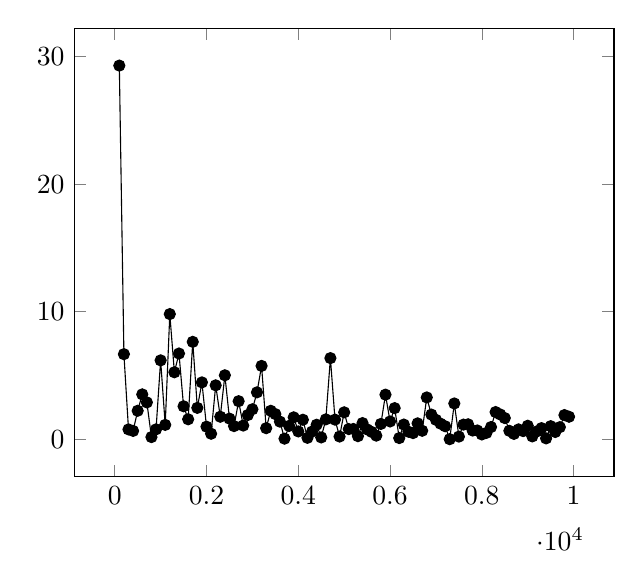
\begin{tikzpicture}
\begin{axis}[%
scatter/classes={%
    a={mark=*,draw=black}}]
\addplot[scatter,%
    scatter src=explicit symbolic]%
table[] {
x y
100 29.3013597131
200 6.67608115296
300 0.776764070439
400 0.658312137375
500 2.23775783256
600 3.52279458509
700 2.89487394893
800 0.174969008885
900 0.780511613849
1000 6.19048494156
1100 1.13028033785
1200 9.81796835074
1300 5.25634019011
1400 6.72721693772
1500 2.59018754531
1600 1.57046855229
1700 7.6409410799
1800 2.4646801547
1900 4.46219854782
2000 0.990014123847
2100 0.436491871283
2200 4.23277221438
2300 1.76976633768
2400 5.02050050307
2500 1.62254311156
2600 1.0355046136
2700 2.98972431033
2800 1.07823342978
2900 1.90257561533
3000 2.35604139525
3100 3.68214719881
3200 5.75517309107
3300 0.872668995946
3400 2.23484131953
3500 1.97801390009
3600 1.38630865303
3700 0.0517417932975
3800 1.04994335262
3900 1.72296632755
4000 0.617362912273
4100 1.53446302427
4200 0.116222445673
4300 0.604327142829
4400 1.14179455157
4500 0.147946253785
4600 1.56366975595
4700 6.36599396891
4800 1.54368140572
4900 0.21574110035
5000 2.11566487836
5100 0.800651910707
5200 0.809479686405
5300 0.24717805459
5400 1.27174602113
5500 0.776764070439
5600 0.577840181246
5700 0.287979656993
5800 1.20676137426
5900 3.50100736713
6000 1.39848685013
6100 2.44465119018
6200 0.0968642972954
6300 1.15615611001
6400 0.594267315013
6500 0.48763351507
6600 1.25021699584
6700 0.669880780466
6800 3.28359014305
6900 1.93853609253
7000 1.52713807636
7100 1.2264705422
7200 1.02565219814
7300 0.00951190134453
7400 2.81007142746
7500 0.211735758566
7600 1.1521013323
7700 1.17709906972
7800 0.688109712897
7900 0.692926056807
8000 0.381579600993
8100 0.505005912255
8200 0.96143234513
8300 2.13716843493
8400 1.94914900455
8500 1.6659943783
8600 0.663751441059
8700 0.425134916356
8800 0.778571612901
8900 0.642858960127
9000 1.06156806724
9100 0.228599207495
9200 0.62091747438
9300 0.87585234131
9400 0.0733068582492
9500 1.03090642932
9600 0.572179715452
9700 0.954462594283
9800 1.90012539338
9900 1.7690285939
    };
\end{axis}
\end{tikzpicture}
\caption{Scatter graph demonstrating the decrease in percentage error based on trials of between 100 and 10,000 samples}
\label{bnaccuracygraph}
\end{figure}

\end{document}